% \textbf{\underline{OZ 3 - De Lorentzkracht en de wet van Ampère - Oefening 4:}}
% \vspace{0.5cm}

% Bereken de kracht die inwerkt op een oneindig lange, rechte draad met stroom $ I $ ten gevolge van:

% \begin{enumerate}[(a)]
%     \item de vierkante spoel in Figuur 3.2.a
%     \item de driehoekige spoel in Figuur 3.2.b
% \end{enumerate}

% \begin{figure}[H]
%     \centering
%     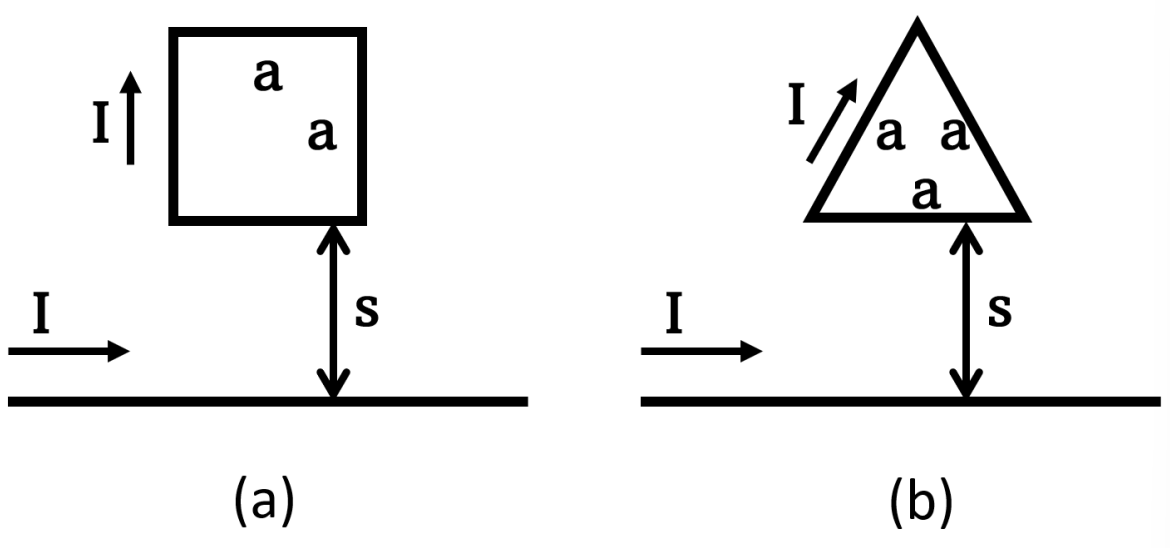
\includegraphics[width=8cm]{oz03/resources/oef-4-opgave.png}
    
%     \textbf{Figuur 3.2}
% \end{figure}

% \begin{description}[labelwidth=1.5cm, leftmargin=!]
%     \item[Geg. :]   $ I $; Zie fig.;
% \end{description}

% \begin{enumerate}[(a)]
%     \item 
%         \begin{description}[labelwidth=1.5cm, leftmargin=!]
%             \item[Gevr. :]  $ F $ bij de vierkante spoel;
%             \item[Opl. :]   TODO
%         \end{description}
%     \item 
%         \begin{description}[labelwidth=1.5cm, leftmargin=!]
%             \item[Gevr. :]  $ F $ bij de driehoekige spoel;
%             \item[Opl. :]   TODO
%         \end{description}
% \end{enumerate}

% \vspace{1cm}